\section{Mock Data}
\label{sect:mock-data}
As most end user's databases are not easily accessible and having control over
the data in databases allows for better testing, generating mock data that is
then loaded into a local database was chosen for ProGENitor development. 
ProGENitor is easily attached to any other databases, so this only speeds up the
development process.  To generate this data, a Perl script was written that
consumes various data files to obtain possible data values and then randomly
selects the values to populate.  The number of users it generates and many other
variables are also controllable.  Once the script completes it outputs a .csv
containing all of the user data, which can be uploaded to the database through
the database architecture included with ProGENitor.

\subsection{Data Files}
To allow for easily updatable mock data, separate data files were implemented,
so that the values weren't embedded deep within the data generation code.  There
are two different types of data files.  The first type simply contains a list
of all possible values.  These values are then simply loaded into an array by
the Generate Data script.  Then, the script will randomly select from this
array when it needs one of these values.  The second type contains a listing of
possible values dependant on a previous value.  For example, in the line below,
to get a Master's Degree in Circuits or Computer Systems, the user must first
obtain a Bachelor's Degree in Electrical.
\\*
\\*Electrical:Circuits,Computer Systems\\*
\\*
Thus, the code will search the second file type for the line that meets the
dependency.  Once the line is found, it will load the possible values into an
array and then randomly select from one of these values.

\subsection{Random Selection}
There are two places the code must randomly select data.  The first is the
data that is loaded for each node.  This random selection simply places the data
from one of the data files into an array and uses the Perl rand function to
randomly select an array index value to pull the data from.  This data is then
applied to the individual user's node and then when the node has all necessary
data generated, it is loaded into the Users.csv file.  This file is then later
uploaded into the database.  In testing, if you want a particular piece of data
to occur more frequently, place it multiple times in the data files and it
will increase the frequency that it will show up in the user data.

The second place that code must randomly select data is when it is determining
if a user enters a node or not on each pass.  There are four possible nodes that
a user could enter each pass and each pass they could potentially enter up to
all of the nodes.  These nodes are an undergraduate degree, a master's degree, a
PhD, and a job.  For each of these nodes, a chance value is assigned in the
variables at the top of the script.  Then essentially a 10 sided dice is rolled
at each node, this is done by loading 1 through 10 into an array and applying
the Perl rand function to the array.  If the dice roll is greater than the
predefined chance value, the node is entered and data is generated.  When any
node is entered, all educational chance values are incremented by 1.  This means
it will be much less likely someone will get an advanced degree as their career
progresses.  Additionally, each educational degree level is currently limited to
one degree and requires the previous level have been completed.  All of these
variables are adjustable in the code; so many different scenarios can be
generated.


\subsection{Code Flow}
Once the data files and random data selection is understood, the code flow is
relatively straight forward.  Essentially, the code just steps through section
by section generating data for each user and loading it into a .csv file that
can later be uploaded into the database.  Figure \ref {fig:data generation}
depicts this process below.

\pagebreak
\usetikzlibrary{shapes,arrows,chains}

\begin{figure}[H]
	\centering
% Start the picture
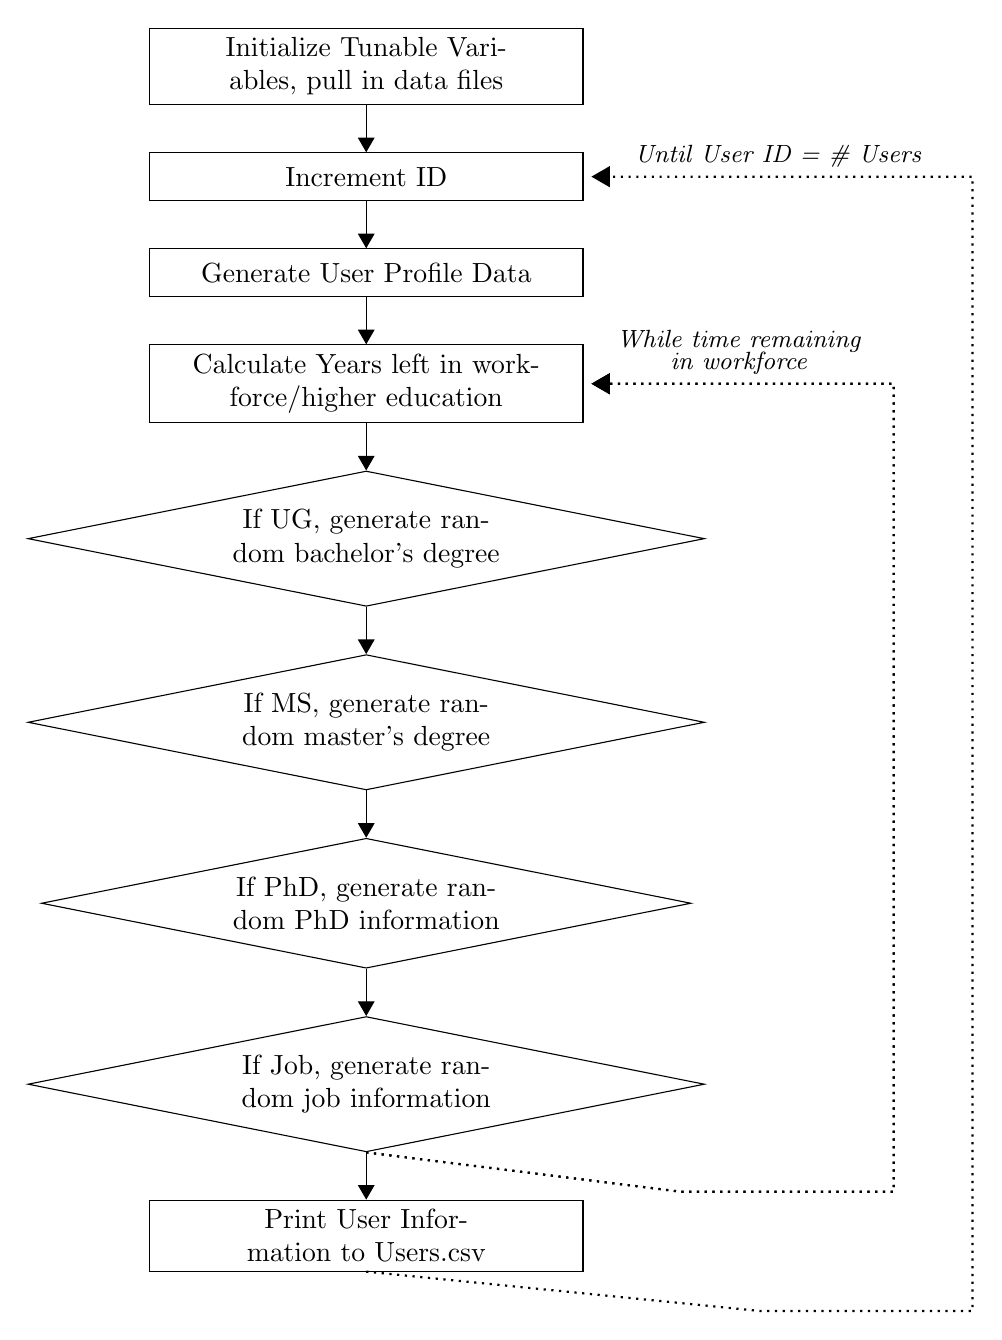
\begin{tikzpicture}[%
    >=triangle 60,              % Nice arrows; your taste may be different
    start chain=going below,    % General flow is top-to-bottom
    node distance=6mm and 60mm, % Global setup of box spacing
    every join/.style={norm},   % Default linetype for connecting boxes
    ]
% ------------------------------------------------- 
% A few box styles 
% <on chain> *and* <on grid> reduce the need for manual relative
% positioning of nodes
\tikzset{
  base/.style={draw, on chain, on grid, align=center, minimum height=4ex},
  proc/.style={base, rectangle, text width=15em},
  test/.style={base, diamond, aspect=5, text width=10em},
  % Connector line styles for different parts of the diagram
  norm/.style={->, draw},
  it/.style={font={\small\itshape}}
}
% -------------------------------------------------
% Start by placing the nodes
\node [proc] (p0) {Initialize Tunable Variables, pull in
data files};
% Use join to connect a node to the previous one 
\node [proc, join] (p1) {Increment ID}; 
\node [proc, join] (p2) {Generate User Profile Data};
\node [proc, join] (p3) {Calculate Years left in workforce/higher education};
\node [test, join] (t0) {If UG, generate random bachelor's degree};
\node [test, join] (t1) {If MS, generate random master's degree};
\node [test, join] (t2) {If PhD, generate random PhD information};
\node [test, join] (t3) {If Job, generate random job information};
\node [proc, join] (p4) {Print User Information to Users.csv};

\draw [->, dotted, thick, shorten >=1mm] (t3.south) -- ++(40mm,-5mm)  --
++(27mm,0) |- node [black, near end, yshift=0.75em, it]
    [above]{While time remaining}(p3);
    
\draw [->, dotted, thick, shorten >=1mm] (t3.south) -- ++(40mm,-5mm)  --
++(27mm,0) |- node [black, near end, yshift=0.75em, it]
    {in workforce}(p3);

\draw [->, dotted, thick, shorten >=1mm]
  (p4.south) -- ++(50mm,-5mm)  -- ++(27mm,0) 
  |- node [black, near end, yshift=0.75em, it]
    {Until User ID = \# Users} (p1);

% -------------------------------------------------
\end{tikzpicture}
	\caption{High Level Data Generation}
	\label{fig:data generation}
\end{figure}